%%%%%%%%%%%%%%%%%%
% 			 
%			Master Thesis - UWB
%				State of the art code
%
%			Author : Wilson Daubry
%
%%%%%%%%%%%%%%%%%%

\chapter{State of the art}
\label{stateoftheart}

This sections has the purpose to explain the state of the art.

\section{Ultra-Wideband Technology}
\label{uwb}
\gls{uwb} is a communication technology using, as the name states, a large bandwidth. This is not a new technology as it is the one used by  Guglielmo Marconi for the first transatlantic communication using radio waves \cite{nekoogar2005uwb}. As define by the \gls{itu-r} to be considered as \gls{uwb}, the bandwidth of communication must be at least 20 \% of the arithmetic center frequency \cite{itur2006characteristics}.
\vspace{2mm}

One interesting feature of \gls{uwb} is the possible coexistence with other radio waves already present in the environment such as \gls{wifi}. As it can be seen on Fig. \ref{fig:UWB_Techonology}, the extension of the \gls{uwb} in the spectral domain is quite huge. 

\begin{figure}[H]
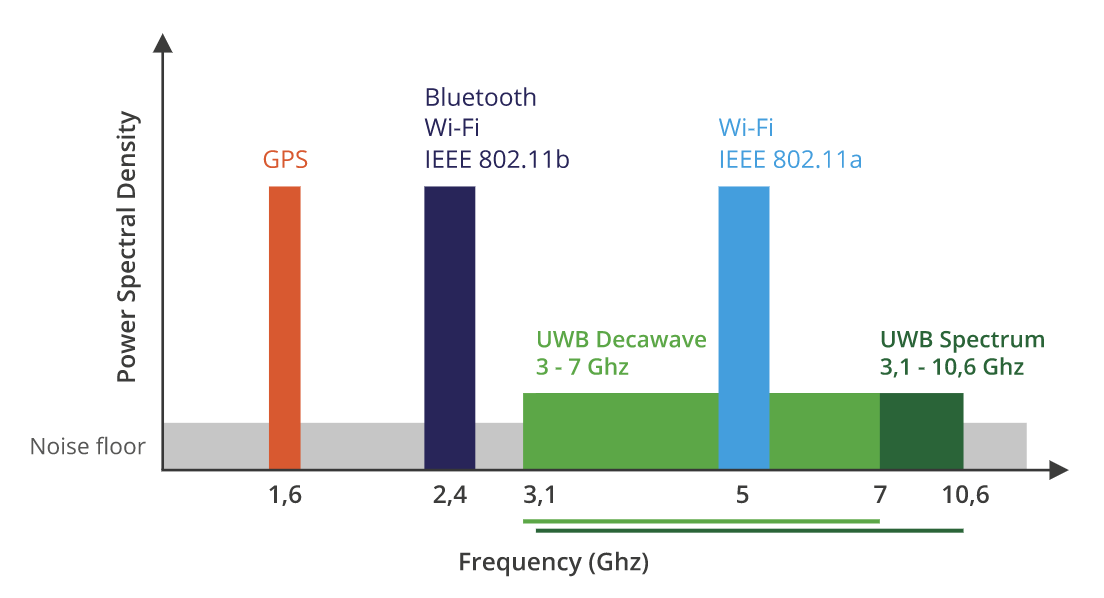
\includegraphics[width=.6\linewidth]{Images/uwb_bandwidth.png}
\centering
\caption{UWB spectrum compared to Wi-Fi and other wireless technology. Taken from \cite{itur2006characteristics}}
\label{fig:UWB_Techonology}
\end{figure} 

Knowing this and based on the time-frequency duality reminded in eq. \ref{fig:eq}, one can see that the extension in the time domain will be quite small.

\begin{equation}
	x(at) \longleftrightarrow \frac{1}{|a|}*X(\frac{f}{a})
\label{fig:eq}
\end{equation}

HERE - ADD THE IMAGE FOR TIME EXTENSION OF UWB

The Fig. \ref{fig:UWB_time} shows the theoretical duration of an impulse of the \gls{uwb}.
% TODO : Ajouter une précision sur la longueur d'une impulsion.

\begin{figure}[H]
\centering
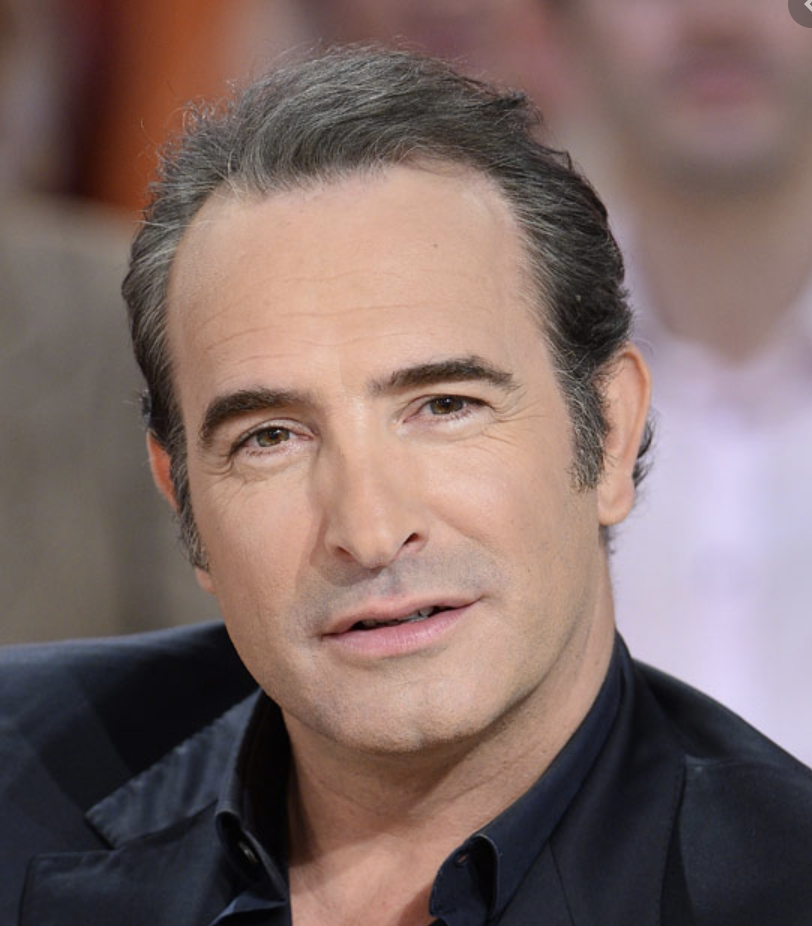
\includegraphics[width=.2\linewidth]{Images/Temporary_pic.png}
\caption{Theoritical duration of an UWB pulse}
\label{fig:UWB_time}
\end{figure}

An advantage of the \gls{uwb} is its robustness in regard of the \gls{mpc}. This can be understood by looking at Fig. \ref{fig:UWB_MPC_Theo}, where several peaks can be distinguished, each corresponding either to a different path travelled by the wave. Indeed, the probability to have a collision depends on the size of the pulse sent. From this, the interest of the \gls{uwb} in confined area appears as a lot of \gls{mpc} are present due to the reflections to all the wall of a room.

\begin{figure}[H]
\centering
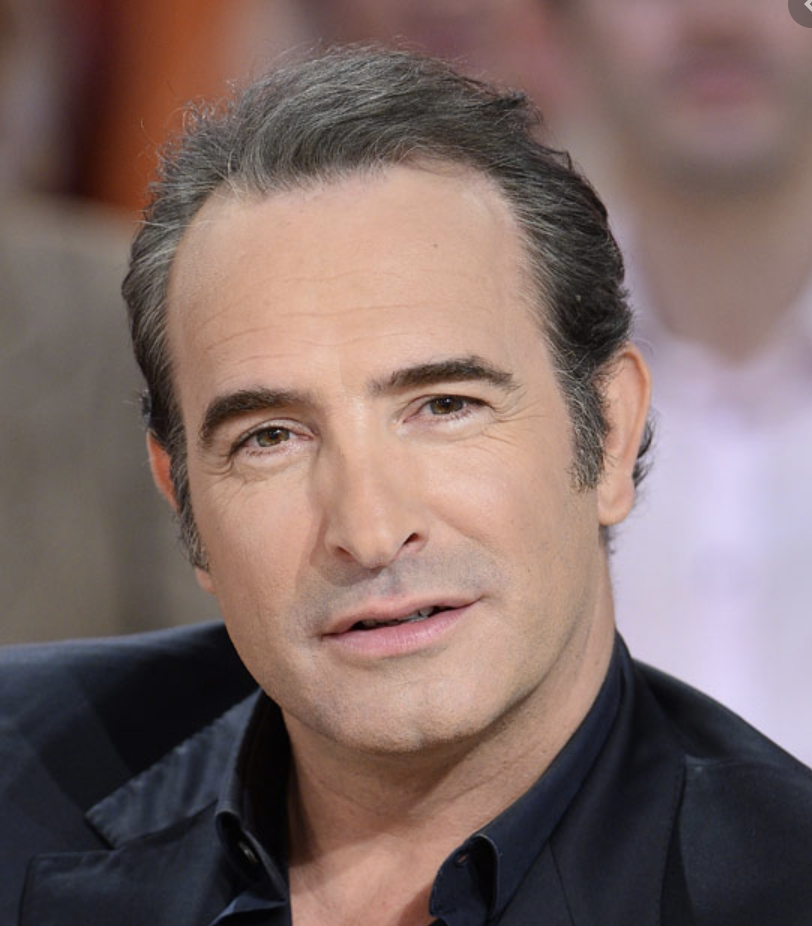
\includegraphics[width=.2\linewidth]{Images/Temporary_pic.png}
\caption{Example of an MPC}
\label{fig:UWB_MPC_Theo}
\end{figure}

\section{Real Time Locating Systems}
\label{rtls}
\gls{rtls} are systems used to track and identify the location of objects in real time. This is a rather vague definition since nothing is specified concerning the means employed to achieve the localization. The \gls{rtls} that will be presented in this section will all have in common the use of wireless communications, between devices being called in this paper "anchor" and "tag". The tag being associated with the object to locate while the anchor is at a fixed and known location.
\vspace{2mm}

Those \gls{rtls} can be separated in two categories : "Relative localization" and "Absolute localization". The relative localization algorithm presented in \ref{sds2wr} is the \gls{tof} method that is used in this project to compute the distance between an anchor and a tag. This choice has been made and explained in \cite{fesler2018high}, \cite{hannotier2019indoor} alongside a presentation of several approach to determine the relative position of a tag relatively to an anchor.

% Faire un lien vers la Thèse de Quentin F entre autre où tout est déjà expliqué et résumé brièvement l'idée.

\subsection{Symmetric double sided two-way ranging}
\label{sds2wr}

\gls{sdstwr} consists in an exchange of three messages between two devices, respectively $RDEV_1$ initiating the communication and `$RDEV_2$. Each device need to save the \gls{toe} or \gls{toa} of every message. Those time being respectively $t_0$, $t_1$ for the first message, $t_2$, $t_3$ for the second message and $t_4$, $t_5$ for the last message.
\vspace{2mm}

Each message contains the different timestamps previously computed, meaning that at the end of this exchange $RDEV_2$ possess all the informations about the timestamps, while $RDEV_1$ misses the last one. If one wants $RDEV_1$ to be able to compute the \gls{tof} then a last message with that $t_5$ in it should be exchanged.
\vspace{2mm}

A schematic of the exchanges between $RDEV_1$ and $RDEV_2$ that occurs in \gls{sdstwr} is shown on Fig. \ref{sdstwr}. 

\begin{figure}[H]
\centering
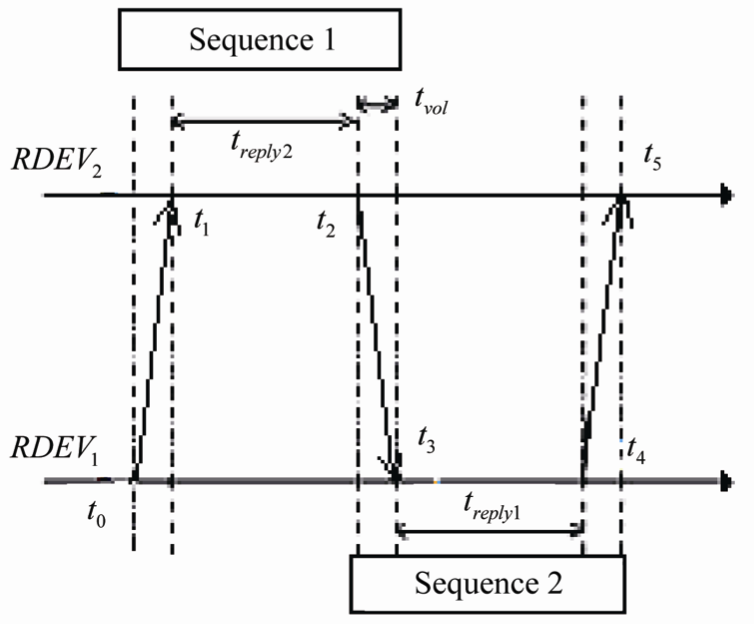
\includegraphics[width=.6\linewidth]{Images/sds-twr.png}
\caption{Symmetric double-sided two-way ranging. Taken from \cite{dalce2011comparison}}
\label{sdstwr}
\end{figure}

Based on those timestamps, the computation of the \gls{tof} can be observed in eq. \ref{fig:tof}.

\begin{equation}
	t_{est} = \frac{((t_3 - t_0) - (t_2 - t_1)) + ((t_5 - t_2) - (t_4 - t_3))}{4}
\label{fig:tof}
\end{equation}

Since that \gls{tof} computed remains an estimation, it is important to know the magnitude of the error as well as its evolution in parallel of the true value of the \gls{tof}.

\begin{equation}
	t_{true} - t_{est} = \frac{1}{4}*(t_{reply2} - t_{reply_1})*(e_1 - e_2)
\end{equation}

The term $e_1 - e_2$ being the difference between the internal clocks of both devices. \cite{dalce2011comparison}

\subsection{Trilateration}

Based on the relative localization performed using \gls{sdstwr}, a \gls{tof} can be computed. If the relative distance between a tag and three different anchors is known, it is possible to compute the intersection of three circle having as center the position of the anchor and radius the \gls{tof} associated to this anchor. A scheme displaying that solution can be seen on Fig. \ref{fig:triangulation}.

\begin{figure}[H]
\centering
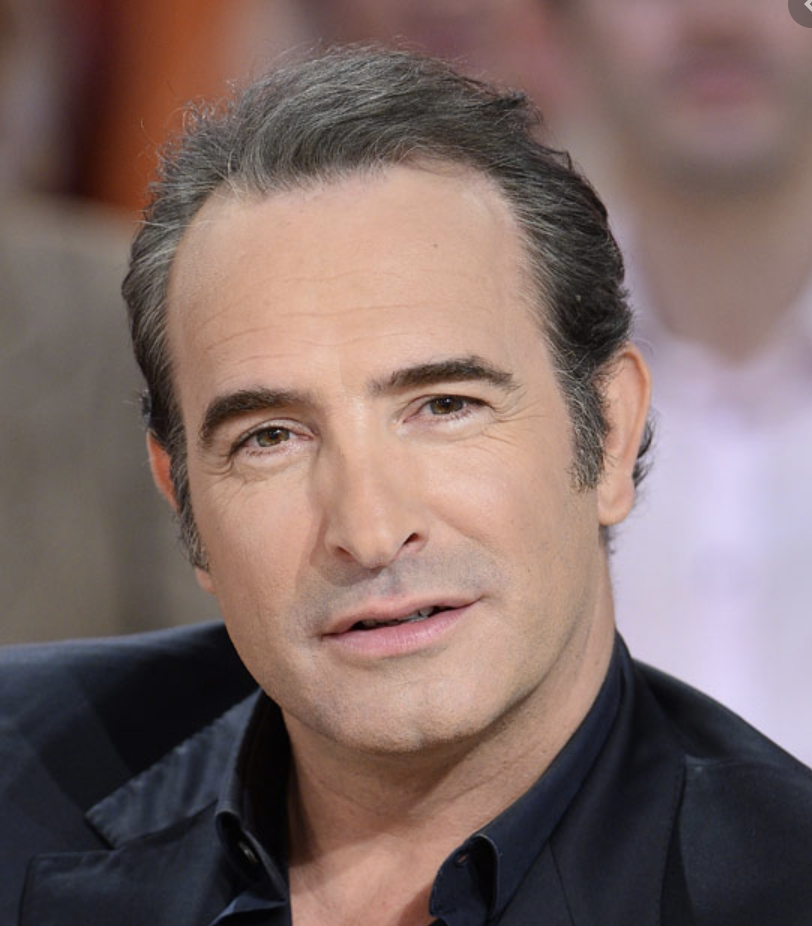
\includegraphics[width=.2\linewidth]{Images/Temporary_pic.png}
\caption{Triangulation -> Ajouter photo}
\label{fig:triangulation}
\end{figure}

As one can deduce, in a two dimensional  plan, three anchors are need to have an intersection of only one point, removing the uncertainty. In a three dimensional plan, four anchors would be needed.
% Rappeler le concept avec un schéma concis. 

\section{Implementation of a locating system}

Using the technology briefly presented in sections \ref{uwb} and \ref{rtls} a locating system has been developed by Quentin Fesler and Cédric Hannotier in  \cite{fesler2018high}, \cite{hannotier2019indoor}. This system is able to retrieve a localization with an error oscillating between twenty and fifty centimetres inside of a building \cite{guyard2019navigation}.
\vspace{2mm}

This locating system is composed of fixed antennas\footnote{Called anchors} made using an ESP8266 as micro-controller and an \gls{uwb} transceiver being the DWM1000 produced by Decawave\cite{decawave}. The tag are built using an Android cellphone, a PSoC \color{red} (get the exact model) \color{black} and also a DWM1000 module.

\subsection{DWM1000}

The DWM1000 is the antenna chosen to operate the wireless communication part, it will be needed for the tag as well as for the different anchors. The configuration of these antenna and the \gls{spi} communication are both explained in this section.

\begin{figure}[H]
	\centering
	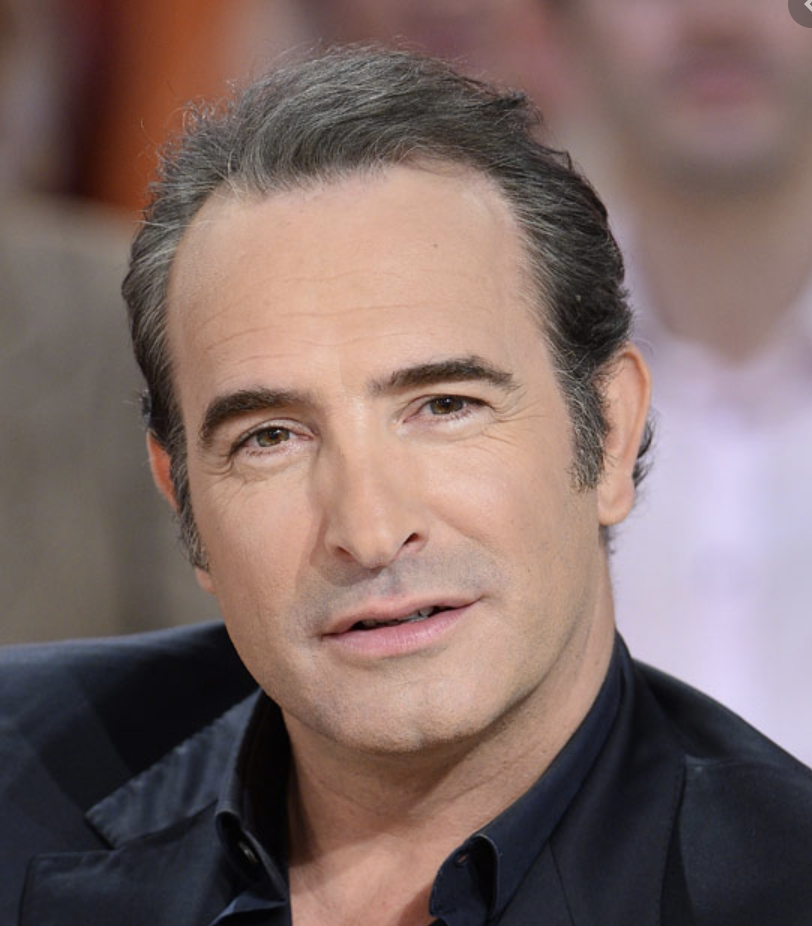
\includegraphics[width=.2\linewidth]{Images/Temporary_pic.png}
	\label{fig:dwm1000}
	\caption{DWM1000 module}
\end{figure}

\subsubsection{Configuration}

Before using the DWM1000, tests have been conducted to choose the most suited configuration to have a low error rate, the  best speed of the communication and the lowest power consumption possible. This leads to the following choices\footnote{A more detailed discussion on the choice of those parameters can be found in \cite{hannotier2019indoor}} :

\begin{itemize}
\item Channel number : 5
\item Bitrate : 6.8 Mbits\textsuperscript{-1}
\item \gls{prf} : 16MHz
\item Preamble length : 128 bits
\end{itemize}

The chosen channel number is the number 5 partly due to the \gls{eu} regulations that are more strict in the frequencies bounds $(3.1; 4.8)$GHz than in the frequencies bounds $(6; 9)$GHz\cite{eulaw}. The other channel that is in those more  boundaries in the $7^{th}$ one. The difference being a bandwidth being twice as large\footnote{The bandwidth of the $5^{th}$ one is 499.2MHz while the one from the $7^{th}$ is 1081.6MHz.}. 
\vspace{2mm}

The choices of the bitrate are restricted between 110kbits\textsuperscript{-1}, 850kbits\textsuperscript{-1} or 6800kbits\textsuperscript{-1}. The reasons behind the choice of the bitrate at 6.8Mbits\textsuperscript{-1} are explained in \cite{hannotier2019indoor}.
\vspace{2mm}

The \gls{prf} can be chosen between 16MHz and 64MHz, an higher one increasing the operating range while consuming more power.
\vspace{2mm}

The preamble length is used for the channel estimation, the longer the more accurate. Unfortunately, a longer preamble means more power consumption unused to transmit "real" data and less time to transmit to "real" data. Recommended bitrate in function of the bitrate are proposed in \cite{usermanual}.
\vspace{2mm}

\subsubsection{Control}

The DWM1000 is piloted via an \gls{spi} bus, this communication follows a master-slave scheme where the master, which is the micro-controller, controls the communication\cite{busspi}. On Fig. \ref{fig:spi_scheme}, the four needed signals are displayed. \gls{miso} and \gls{mosi} are the connections used to transmit the data between the master and its slave.
The \gls{sckl}, generated by the master fixes the transmission speed happening on the \gls{miso} and \gls{mosi}.  Since the \gls{spi} allows different slaves for only one master, the \gls{ss} is used by the master to select a specific slave to communicate with. 

\begin{figure}[H]
	\centering
	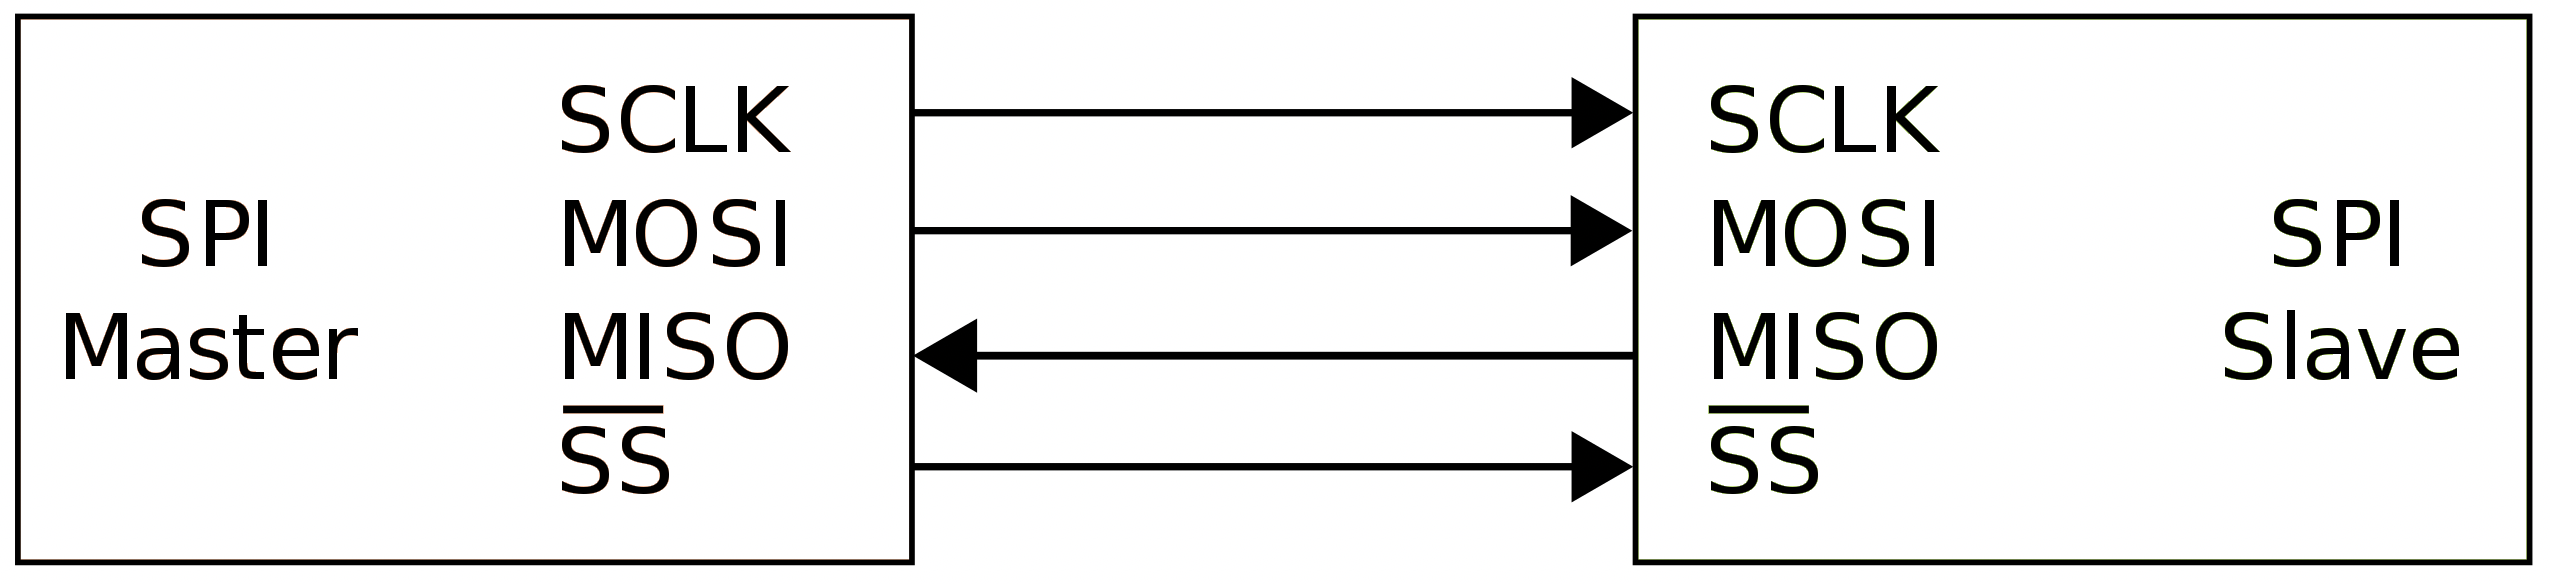
\includegraphics[width=.6\linewidth]{Images/SPI_scheme.png}
	\caption{SPI Schematic}
	\label{fig:spi_scheme}
\end{figure}

\subsection{Anchor}

The anchors are fixed antennas composed of a DWM1000 and an ESP8266 \cite{esp8266}. They are placed at known position in the room and are used to compute the \gls{tof} between the tag and the anchor using the \gls{sdstwr} explained in section \ref{sds2wr}. 

\begin{figure}[H]
	\centering
	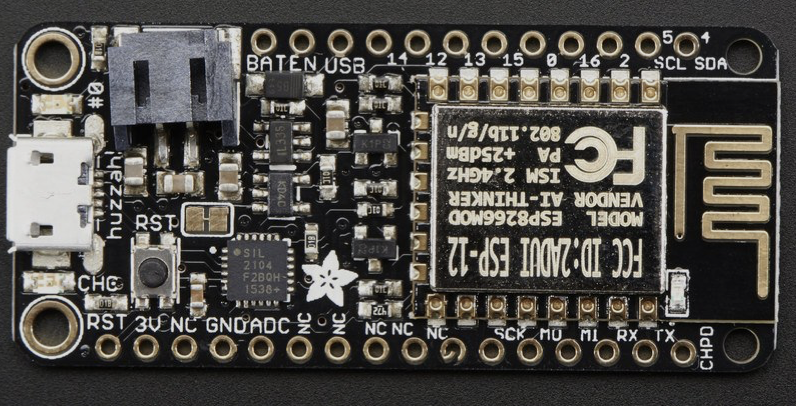
\includegraphics[width=.6\linewidth]{Images/esp8266.png}
	\caption{ESP8266 mounted on a Feather Huzzah board. Taken from \cite{adafruit}}
	\label{fig:esp8266}
\end{figure}

The micro-controller has been combined with the development board Feather Huzzah from Adafruit \cite{adafruit}, the Fig. \ref{fig:esp8266} represents this module. This board can be flashed using an USB serie connection, allowing a easy deployment of the code, it also have the advantage to be light and small, an useful feature to deploy several anchors in a room without much cluttering.

\subsection{Tag}

The tag is the object we want to know the localization. It is composed of a DWM1000 antenna, a PSoC\footnote{The exact model is the : CY8C5888LTI-LP097 \cite{guyard2019navigation}} and an Android application. The Fig. \ref{fig:psoc} shows the PSoC used as well as its custom board made by the electronic BEAMS service of the ULB.
\vspace{2mm}

\begin{figure}[H]
	\centering
	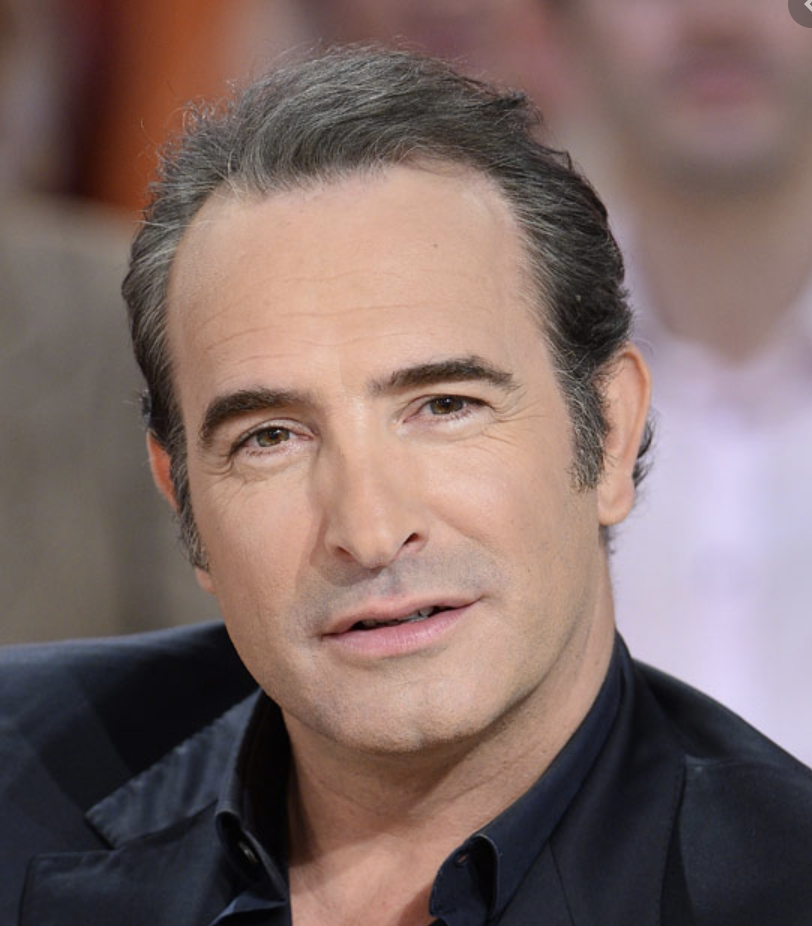
\includegraphics[width=.2\linewidth]{Images/Temporary_pic.png}
	\caption{PSoC card}
	\label{fig:psoc}
\end{figure}

The communication between the DWM1000 an the PSoC is performed using a \gls{spi} bus as for the anchors, the PSoC being the master. As for the ESP8266, the PSoC can flashed through an USB bus. The micro-controller receives instructions from the application on the cellphone and controls the communications of the DWM1000 with the different anchors. It then transmits the received data from the DWM1000 to the application through a USB bus. \color{red} Verifier que c'est bien un USB bus \color{black}.

\subsection{Android Application}

To control t



\subsection{Communication protocol}

A schematic of the execution 

\begin{figure}[H]
\centering
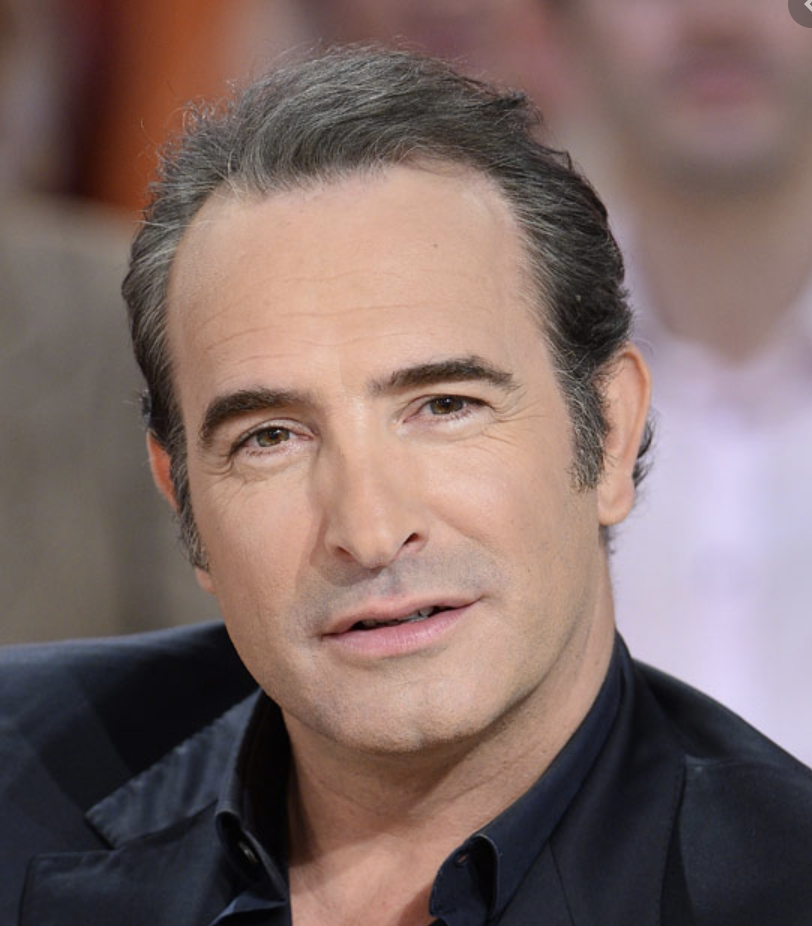
\includegraphics[width=.2\linewidth]{Images/Temporary_pic.png}
\caption{Communication protocol -> Ajouter photo}
\label{fig:com_prot}
\end{figure}


% L'objectif de cette section est de faire part au lecteur de l'avancement du projet au moment où je l'ai prit en main.
% Points à aborder : Matériel utilisé, précision obtenue

\section{Virtual Anchor}

% La on attaque la partie dure. Parler des ancres virtuelles, introduire le concept avec des schémas, montrer qu'on à dès lors besoin de la CIR.
% Parler des articles qui expliquent la théorie avec du MPC.